\documentclass{article}
\usepackage{graphicx}
\usepackage{enumitem}
\usepackage{xcolor}
\usepackage{pifont} % Pour les symboles (croix)
\usepackage{pseudocode}
\usepackage{listings}
\usepackage[colorlinks=true,linkcolor=blue,urlcolor=blue,citecolor=blue]{hyperref}

\lstset{
    language=C,
    basicstyle=\ttfamily,
    keywordstyle=\color{blue},
    commentstyle=\color{green!60!black},
    stringstyle=\color{red},
    numbers=left,
    numberstyle=\tiny\color{gray},
    breaklines=true,
    literate=
    {à}{{\'a}}1 
    {è}{{\`{e}}}1
    {î}{{\^i}}1
    {ê}{{\^e}}1
    {ù}{{\`u}}1
    {é}{{\'e}}1,
    showstringspaces=false,
    frame=single,
    tabsize=2
}

\begin{document}

\title{Rapport de projet ALGO}

{\centering
\author{Achraf,Thomas,Elouen,Woody}
\par}
\date{Janvier 2024}
\maketitle


\thispagestyle{empty}

\newpage

\tableofcontents

\newpage

\maketitle

\section{\textbf{Introduction}}

Ce projet avait pour but de développer un compresseur / décompresseur qui utilise l'algorithme d'Huffman pour compresser et décompresser un fichier. Ce compresseur fonctionne en trasformant des caractères en bits, habituellement codés sur plusieurs octets.  Au cours de ce développement, nous mettrons en place les étapes du cycle en V afin de réaliser au mieux le projet. Le langage de programmation utilisé est le C. Pour ce projet, nous avons respecté un planning donné sur Moodle : 
-Mardi 24/10 - Analyse : spécification des TAD
-Mardi 7/11 - Analyse : analyse descendante des opérations métiers
-Mardi 14/11 - Conception préliminaire
-Mardi 21/11 - Conception détaillée
-Mardi 28/11 - Développement et tests unitaires
-Mardi 5/12 - Développement et tests unitaires
-Mardi 12/12 - Debogage et rapport
-Mardi 9/1 - Dépôt des projets sur moodle
-Vendredi 12/1 - Soutenances
En plus de ces séances de projet, notre groupe se réunissait souvent afin d'avancer conjointement sur l'écriture et le développement du projet. La suite de ce rapport comportera l'ensemble des TAD, conceptions et programmes nous ayant permis de faire aboutir le développement de ce compresseur.


\newpage


\section{\textbf{Analyses}}

\subsection{Compression}

\begin{figure}[h!]
  \centering
  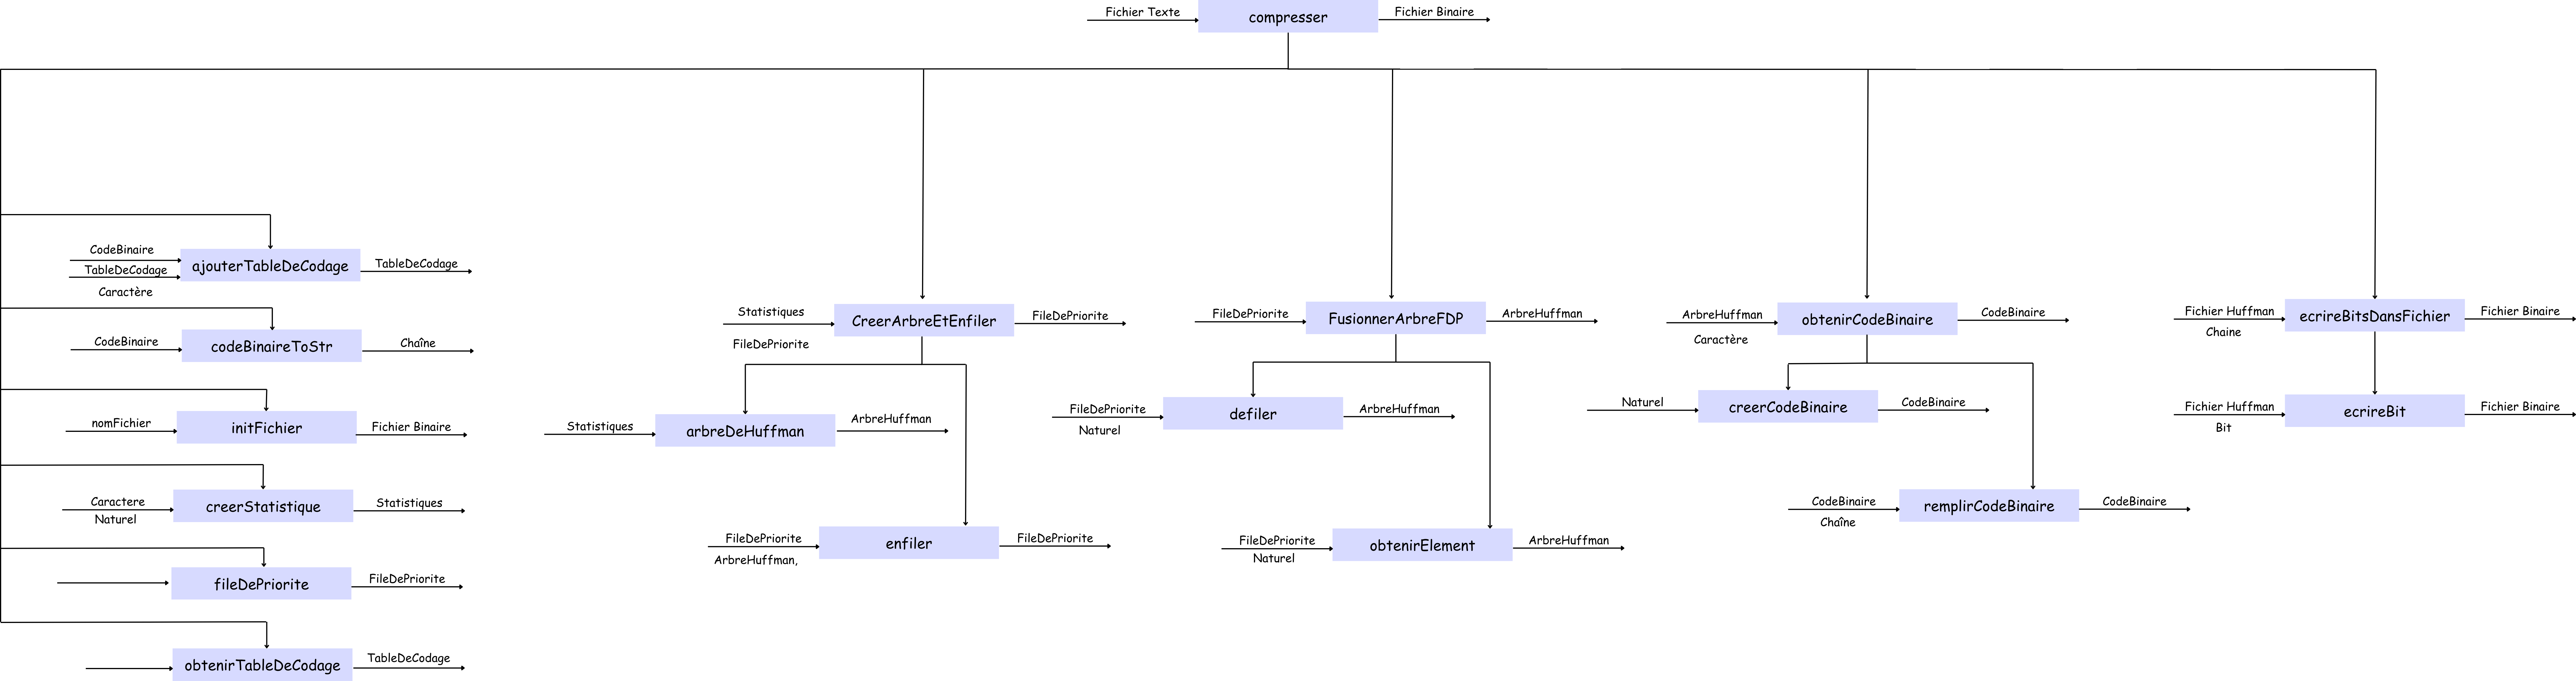
\includegraphics[width=1.3\linewidth]{./images/Analyse_Descendante_Compression.png}
  \caption{Analyse Descendante Compression}
  \label{fig:AD_Comp}
\end{figure}


\subsection{Decompression}


\begin{figure}[h!]
  \centering
  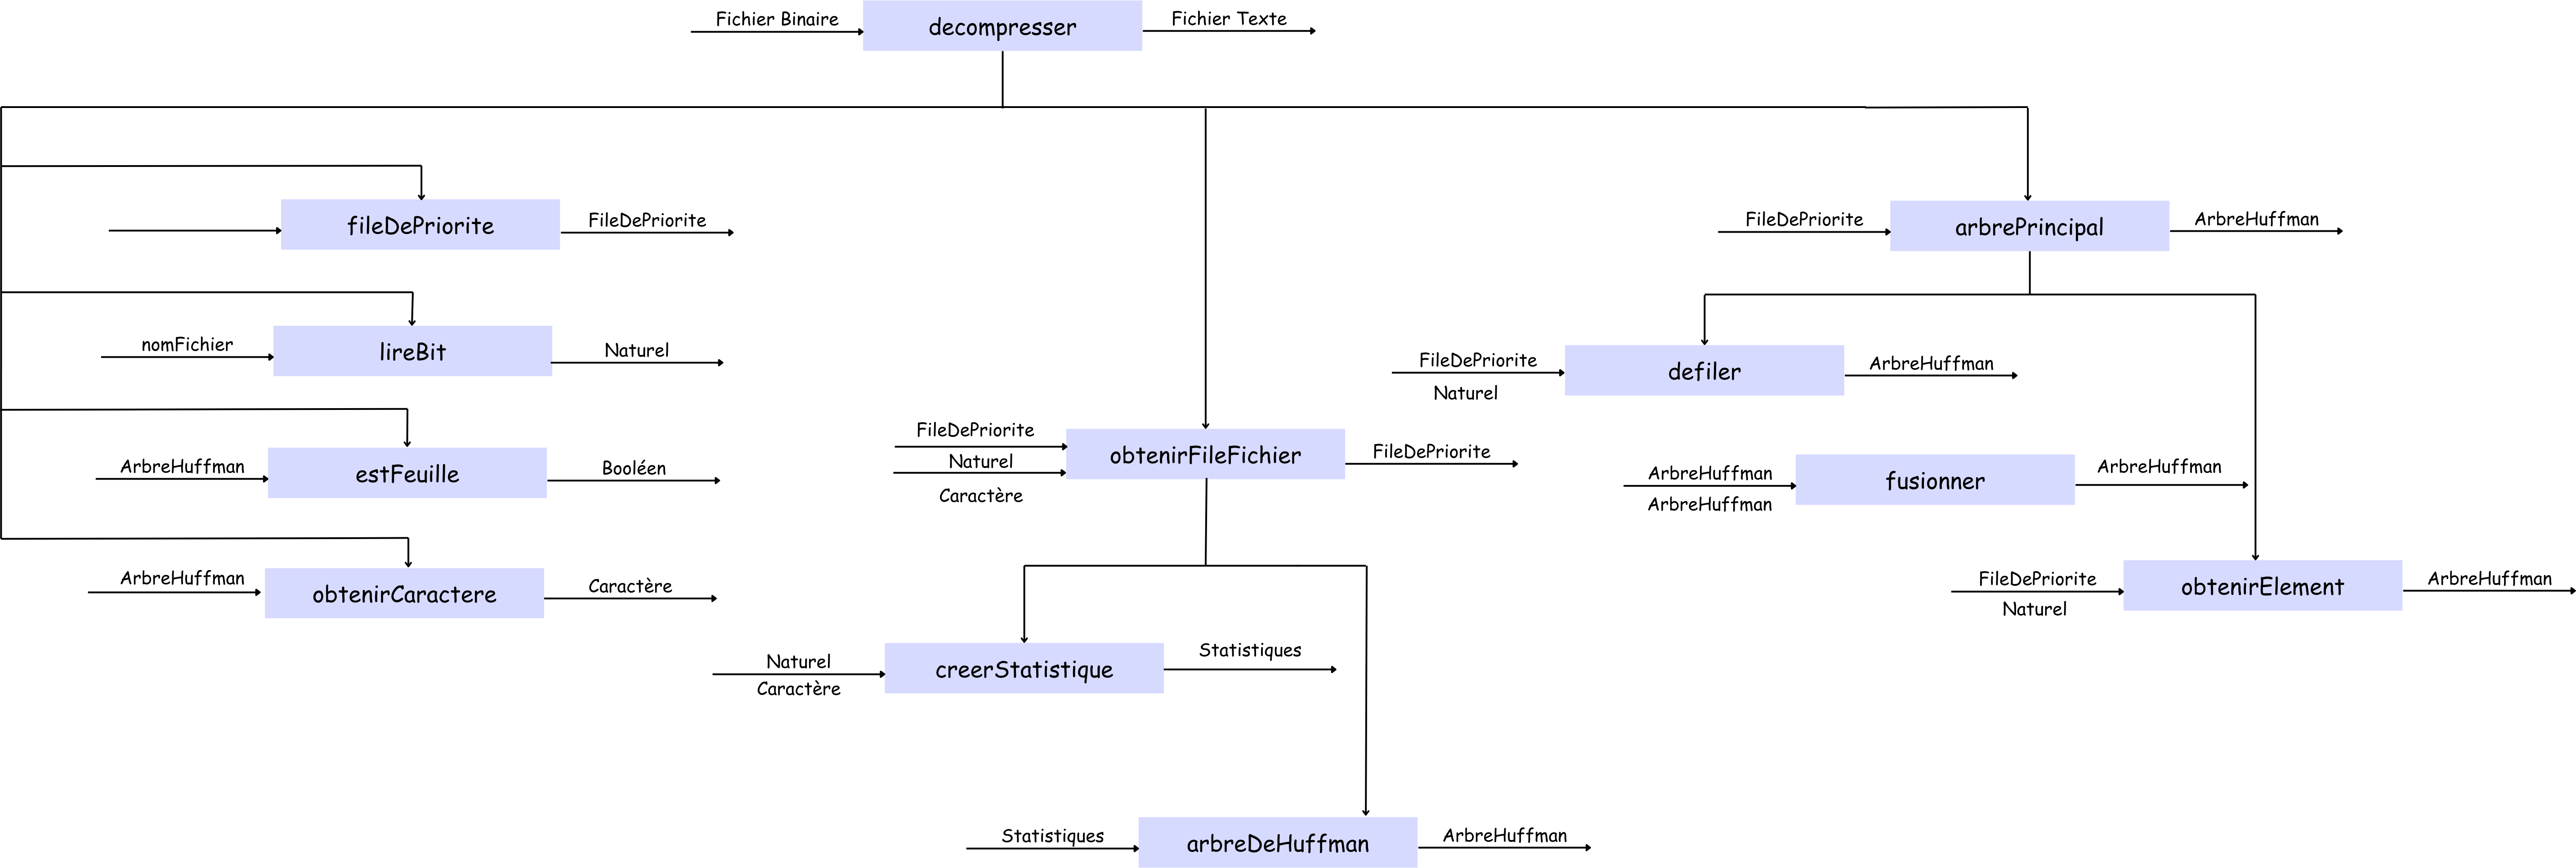
\includegraphics[width=1.3\linewidth]{./images/Analyse_Descendante_Decompression.png}
  \caption{Analyse Descendante Décompression}
  \label{fig:AD_Decomp}
\end{figure}

\subsection{TAD Code Binaire}
\begin{tad}
\tadNom{Code Binaire}
        
\tadDependances{TableDeCodage, Caractere, Bit}
\begin{tadOperations}{obtenirCodeBinaireR}
    \tadOperation{creerCodeBinaire}{\tadParams{\naturel}}{\tadParams{CodeBinaire}}
    \tadOperationAvecPreconditions{remplirCodeBinaire}{\tadDeuxParams{\chaine}{CodeBinaire}}{\tadParams{CodeBinaire}}
    \tadOperation{libererCodeBinaire}{\tadParams{CodeBinaire}}{\tadParams{CodeBinaire}}
    \tadOperation{estVide}{\tadParams{CodeBinaire}}{\tadParams{\booleen}}
    \tadOperationAvecPreconditions{obtenirIemeBit}{\tadParams{CodeBinaire,\naturelNonNul}}{\tadParams{Bit}}
    \tadOperation{longueur}{\tadParams{CodeBinaire}}{\tadParams{\naturel}}
    \tadOperation{concatener}{\tadDeuxParams{CodeBinaire}{CodeBinaire}}{\tadParams{CodeBinaire}}
    \tadOperation{codeBinaireToStr}{\tadParams{CodeBinaire}}{\tadParams{\chaine}}
    \tadOperationAvecPreconditions{obtenirCodeBinaire}{\tadDeuxParams{ArbreHuffman}{\caractere}}{\tadParams{\chaine}}
    \tadOperationAvecPreconditions{obtenirCodeBinaireR}{\tadDeuxParams{ArbreHuffman}{\caractere}}{\tadParams{\chaine}}
    \tadOperation{CbFromAH}{\tadDeuxParams{ArbreHuffman}{\caractere}}{\tadParams{CodeBinaire}}        
    \tadOperation{codeBinaireToStr}{\tadParams{CodeBinaire}}{\tadParams{\chaine}}
\end{tadOperations}
\begin{tadSemantiques}{obtenirCodeBinaireR}
    \tadSemantique{creerCodeBinaire}{Fonction qui creer un code binaire à partir de sa taille}
    \tadSemantique{remplirCodeBinaire}{Fonction qui permet de remplir un code binaire avec une chaîne de caractère}
    \tadSemantique{libererCodeBinaire}{Fonction qui libère un code binaire }
    \tadSemantique{estVide}{Fonction qui permet de savoir si un code est vide ou non}
    \tadSemantique{obtenirIemeBit}{Fonction qui permet d'obtenir le ieme bit d'un code binaire}
    \tadSemantique{concatener}{Fonction qui permet de concatener 2 codes binaires}
    \tadSemantique{codeBinaireToStr}{Fonction qui permet de convertir un code binaire en chaîne de caractères}
    \tadSemantique{obtenirCodeBinaire}{Fonction qui va permettre d'avoir le code binaire d'un caractere}
    \tadSemantique{obtenirCodeBinaireR}{Fonction récursive qui va permettre d'avoir le code binaire d'un caractere et qui va être appelé dans obtenirCodeBinaire}
    \tadSemantique{CbFromAH}{Fonction qui donne un code binaire à partir d'un arbre d'Huffman et d'un caractere }
    \tadSemantique{codeBinaireToStr}{Fonction qui transforme un code binaire en chaine de caracteres}
\end{tadSemantiques}
\begin{tadPreconditions}{obtenirCodeBinaireR(a, car)}
        \tadPrecondition{remplirCodeBinaire(code)}{$longueur(chaine) \ne code.taille$}
        \tadPrecondition{obtenirIemeBit(code, i)}{$i > 0$ et $i \leq longueur(code)$}
        \tadPrecondition{obtenirCodeBinaire(a, car)}{non ArbreHuffman.estVide(a)}
        \tadPrecondition{obtenirCodeBinaireR(a, car)}{non ArbreHuffman.estVide(a)}
\end{tadPreconditions}
\end{tad} 

\subsection{TAD Octet}
\begin{tad}
\tadNom{Octet}

\tadDependances{Chaine de caracteres, Code Binaire, Booleen, Bit}
\begin{tadOperations}{ObtenirOctet}
    \tadOperation{creerOctet}{}{\tadParams{Octet}}
    \tadOperation{fixerBit}{\tadParams{Octet}{\entier}{Bit}}{\tadParams{Octet}}
    \tadOperation{iemeBit}{\tadParams{Octet}{\entier}}{Bit}
    \tadOperation{decaler}{\tadParams{Octet}}{Octet}
    \tadOperation{bitsToStr}{\tadParams{Octet}}{\chaine}
    \tadOperation{strToBits}{\chaine}{Octet}
    \tadOperationAvecPreconditions{encoder}{\tadDeuxParams{Octet}{Code Binaire}}{Octet}
    \tadOperation{estVide}{\tadParams{Octet}}{\booleen}
    \tadOperation{inverser}{\tadParams{Octet}}{Octet}
\end{tadOperations}
\begin{tadSemantiques}{obtenirCodeBinaire}
    \tadSemantique{creerOctet}{Permet d'obtenir un octet avec tous ses bits à 0}
    \tadSemantique{fixerBit}{Permet de fixer les bits d'un octet}
    \tadSemantique{iemeBit}{Renvoie le i-eme bit d'un octet}
    \tadSemantique{decaler}{Decale l'octet vers la gauche}
    \tadSemantique{bitsToStr}{Renvoie un octet en chaîne de caractere}
    \tadSemantique{strToBits}{Renvoie l'octet d'une chaîne de caractere}
    \tadSemantique{encoder}{Remplit un octet avec un code binaire}
    \tadSemantique{estVide}{Verfie si l'octet est vide}
    \tadSemantique{inverser}{Inverse l'octet}

    
\end{tadSemantiques}
\begin{tadPreconditions}{decoder(code, chaine)}
    \tadPrecondition{encoder(o, code,i)}{non estVide(code), $0 \leq i \leq 7$}
\end{tadPreconditions}
\end{tad}
    
\subsection{TAD Statistiques}
\begin{tad}
\tadNom{Statistiques}
\tadDependances{Caractère, Chaine de caracteres, Naturel}
\begin{tadOperations}{statistiques}
    \tadOperation{statistiques}{\tadDeuxParams{\caractere}{\naturel}}{\tadParams{ Statistiques}}
    \tadOperation{obtenirOccurences}{\tadParams{Statistiques}}{\tadParams{\naturel}}
    \tadOperation{obtenirCaractere}{\tadParams{Statistiques}}{\tadParams{\caractere}}
\end{tadOperations}
\begin{tadSemantiques}{}
    \tadSemantique{statistiques}{Créer une statistique à partir d'un caractère et d'un naturel}\newline
    \tadSemantique{obtenirOccurences}{Permet d'obtenir le nombre d'occurences d'une statistique}\newline
    \tadSemantique{obtenirCaractere}{Permet d'obtenir le caractère d'une statistique}\newline
\end{tadSemantiques}                     
\end{tad}



\subsection{TAD ArbreHuffman}
\begin{tad}
\tadNom{ArbreHuffman}
\tadDependances{statistiques,\booleen}
\begin{tadOperations}{obtenirPonderation}
    \tadOperation{arbreDeHuffman}{Statistiques}{\tadParams{ArbreHuffman}}
    \tadOperation{fixerStatistique}{\tadDeuxParams{ArbreHuffman}{Statistiques}}{\tadParams{ArbreHuffman}}
    \tadOperation{obtenirStat}{\tadParams{ArbreHuffman}}{\tadParams{Statistiques}}
    \tadOperation{obtenirCaractere}{ArbreHuffman}{\tadParams{\caractere}}
    \tadOperationAvecPreconditions{fusionner}{\tadDeuxParams{ArbreHuffman}{ArbreHuffman}}{\tadParams{ArbreHuffman}}
    \tadOperation{obtenirPonderation}{\tadParams{ArbreHuffman}}{\tadParams{\naturel}}
    \tadOperationAvecPreconditions{fixerFilsDroit}{\tadDeuxParams{ArbreHuffman}{Arebre Huffman}}{\tadParams{ArbreHuffman}}
    \tadOperationAvecPreconditions{fixerFilsGauche}{\tadDeuxParams{ArbreHuffman}{Arebre Huffman}}{\tadParams{ArbreHuffman}}
    \tadOperationAvecPreconditions{obtenirFilsGauche}{\tadParams{ArbreHuffman}}{\tadParams{ArbreHuffman}}
    \tadOperationAvecPreconditions{obtenirFilsDroit}{\tadParams{ArbreHuffman}}{\tadParams{ArbreHuffman}}
    \tadOperation{estFeuille}{\tadParams{ArbreHuffman}}{\tadParams{\booleen}}
    \tadOperation{estVide}{\tadParams{ArbreHuffman}}{\tadParams{\booleen}}
    \tadOperation{estPresent}{\tadParams{ArbreHuffman}}{\tadParams{\booleen}}
    \tadOperationAvecPreconditions{copierArbreHuffman}{\tadParams{ArbreHuffman}}{\tadParams{ArbreHuffman}}
\end{tadOperations}
\begin{tadSemantiques}{obtenirPonderation}
    \tadSemantique{arbreDeHuffman}{Crée un arbre de huffman à partir d'une statistique}
    \tadSemantique{fixerStatistique}{Fixe une statistique à un arbre}
    \tadSemantique{obtenirStat}{Retourne la valeur de la statistique d'un arbre}
    \tadSemantique{obtenirCaractere}{Retourne le caractère associé à un arbre}
    \tadSemantique{fusionner}{Fusionne deux arbres entre eux}
    \tadSemantique{obtenirPonderation}{Permet d'obtenir la ponderation d'un arbre de huffman}
    \tadSemantique{fixerFilsDroit}{Affecte la valeur au fils droit de l'arbre}
    \tadSemantique{fixerFilsGauche}{Affecte la valeur au fils gauche de l'arbre}
    \tadSemantique{obtenirFilsGauche}{Permet d'obtenir le fils gauche d'un arbre de huffman}
    \tadSemantique{obtenirFilsDroit}{Permet d'obtenir le fils droit d'un arbre de huffman}
    \tadSemantique{estFeuille}{Verifie si l'arbre de huffman est une feuille}
    \tadSemantique{estVide}{Verifie si l'arbre est vide, si son champ caractère est vide}
    \tadSemantique{estPresent}{Vérifie si un élément est présent dans un arbre}
    \tadSemantique{copierArbreHuffman}{Fonction qui permet de copier un arbre}
\end{tadSemantiques}
\begin{tadPreconditions}{obtenirFilsGauche(A)}
    \tadPrecondition{fusionner(A)}{estVide(A)}
    \tadPrecondition{fixerFilsDroit(r,ad)}{non(estVide(r))}
    \tadPrecondition{fixerFilsGauche(r,ag)}{non(estVide(r))}
    \tadPrecondition{obtenirFilsGauche(A)}{non estUneFeuille(A)}
    \tadPrecondition{obtenirFilsDroit(A)}{non estUneFeuille(A)}
    \tadPrecondition{copierArbreHuffman(arbre)}{arbre $\ne$ NULL}
\end{tadPreconditions}
\end{tad}


\subsection{FileDePriorité}
\begin{tad}
\tadNom{FileDePriorité} 
\tadDependances{Booleen} 
\begin{tadOperations}{fileDePriorite}
    \tadOperation{fileDePriorite}{}{\tadParams{FileDePriorite}}
    \tadOperation{enfiler}{\tadDeuxParams{FileDePriorite}{Element}}{\tadParams{FileDePriorite}}
    \tadOperation{defiler}{\tadParams{FileDePriorite}}{\tadParams{FileDePriorite}}
    \tadOperation{longueur}{\tadParams{FiledePriorite}}{\tadParams{\naturel}}
    \tadOperation{estVide}{\tadParams{FileDePriorite}}{\tadParams{\booleen}}
    \tadOperation{estPresent}{\tadDeuxParams{FileDePriorite}{Element}}{\tadParams{\booleen}}
    \tadOperation{obtenirElement}{\tadParams{FileDePriorite}}{\tadParams{Element}}
\end{tadOperations}
\begin{tadSemantiques}{fileDePriorite}
    \tadSemantique{filedePriorite}{Créer une file de priotité vide}
    \tadSemantique{enfiler}{Enfile un élément en fin de file}
    \tadSemantique{defiler}{Défile le dernier élément de la file}
    \tadSemantique{longueur}{Calcule la longueur de la file}
    \tadSemantique{estVide}{Cherche si la file de priotité est vide ou non}
    \tadSemantique{estPresent}{Cherche si un élément donné est présent dans la file ou non}
    \tadSemantique{obtenirElement}{Donne le dernier élément de la file}
\end{tadSemantiques}
\end{tad}

\subsection{TAD TableDeCodage}
\begin{tad}
\tadNom{TableDeCodage}
\tadDependances{ArbreHuffmann}
\begin{tadOperations}{obtenirTableDeCodage}
    \tadOperation{obtenirTableDeCodage}{\tadParams{ArbreHuffman}}{\tadParams{TableDeCodage}}
    \tadOperationAvecPreconditions{obtenirCode}{\tadDeuxParams{TableDeCodage}{\caractere}}{\tadParams{CodeBinaire}}
    \tadOperation{obtenirCarac}{\tadDeuxParams{TableDeCodage}{CodeBinaire}}{\tadParams{\caractere}}
    \tadOperation{ajouter}{\tadDeuxParams{\tadDeuxParams{TableDeCodage}{caractere}}{CodeBinaire}}{\tadParams{TableDeCodage}}
    \tadOperation{retirer}{\tadDeuxParams{TableDeCodage}{\caractere}}{\tadParams{TableDeCodage}}
    \tadOperation{estPresent}{\tadDeuxParams{TableDeCodage}{\caractere}}{\tadParams{\booleen}}
    \tadOperation{estVide}{\tadParams{TableDeCodage}}{\tadParams{\booleen}}
\end{tadOperations}
\begin{tadSemantiques}{obtenirTableDeCodage}
    \tadSemantique{obtenirTableDeCodage}{Renvoie la table de codage grâce à un arbre de Huffman}\newline
    \tadSemantique{obtenirCode}{Permet d'obtenir le code binaire d'un caractère grâce à la TableDeCodage}\newline
    \tadSemantique{obtenirCarac}{Permet d'obtenir le caractere d'un code binaire grâce à la TableDeCodage}\newline
    \tadSemantique{ajouter}{Permet d'ajouter une nouveeau caractère avec son code binaire dans la TableDeCodage}\newline
    \tadSemantique{supprimerer}{Permet de supprimer un caractère de la TableDeCodage}\newline
    \tadSemantique{estPresent}{Permet de savoir si un caractère est présent dans la TableDeCodage}\newline
    \tadSemantique{estVide}{Permet de savoir si la TableDeCodage est vide}\newline
\end{tadSemantiques}
\begin{tadPreconditions}{obtenirTableDeCodage(A)}
    \tadPrecondition{obtenirTableDeCodage(A)}{non estVide(A)}
    \tadPrecondition{obtenirCode(t,c)}{estPresent(t,c)}
\end{tadPreconditions}
\end{tad}










\newpage

\section{Conception préliminaire}

\subsection{\textbf{Arbre Huffman}}

\begin{algorithme}
\signatureFonction{arbreDeHuffman}
	{stat : Statistiques}{\typePointeur{ArbreHuffman}}
	{}
\end{algorithme}

\begin{algorithme}
\signatureProcedure{fixerStatistique}{\paramEntreeSortie{arbre : \typePointeur{ArbreHuffman}} \paramEntree{stat : Statistiques}}
	{}	
\end{algorithme}

\begin{algorithme}
	\signatureFonction{obtenirStat}{arbre : ArbreHuffman}{Statistiques}
	{}		
\end{algorithme}

\begin{algorithme}
	\signatureFonction{obtenirPonderation}{arbre : ArbreHuffman}{\naturel}
	{}	
\end{algorithme}

\begin{algorithme}
	\signatureFonction{obtenirCaractere}{arbre : ArbreHuffman}{\caractere}
	{}	
\end{algorithme}

\begin{algorithme}
\signatureFonction{fusionner}{arbre1, arbre2 : \typePointeur{ArbreHuffman}}{\typePointeur{ArbreHuffman}}
	{non estVide(arbre1) ou non estVide(arbre2)}
\end{algorithme}

\begin{algorithme}
	\signatureProcedure{fixerFilsGauche}{\paramEntreeSortie{arbre : \typePointeur{ArbreHuffman}}, \paramEntree{gauche : \typePointeur{ArbreHuffman}}}
	{}
\end{algorithme}
		
\begin{algorithme}
	\signatureProcedure{fixerFilsDroit}{\paramEntreeSortie{arbre : \typePointeur{ArbreHuffman}}, \paramEntree{droit : \typePointeur{ArbreHuffman}}}
	{}
\end{algorithme}

\begin{algorithme}
\signatureFonction{estFeuille}{arbre : Arbre Huffman}{\booleen}
	{}
\end{algorithme}

\begin{algorithme}
\signatureFonction{estVide}{arbre: \typePointeur{ArbreHuffman}}{\booleen}
	{}
\end{algorithme}

\begin{algorithme}
\signatureFonction{obtenirFilsGauche}{arbre : \typePointeur{ArbreHuffman}}{\typePointeur{ArbreHuffman}}
	{non estFeuille(arbre)}
\end{algorithme}

\begin{algorithme}
\signatureFonction{obtenirFilsDroit}{arbre : \typePointeur{ArbreHuffman}}{\typePointeur{ArbreHuffman}}
	{non estFeuille(arbre)}
\end{algorithme}

\begin{algorithme}
	\signatureFonction{estPresent}{arbre : \typePointeur{ArbreHuffman}, caractere : \caractere}{\booleen}
	{}
\end{algorithme}

\begin{algorithme}
	\signatureFonction{copierArbreHuffman}{arbre : \typePointeur{ArbreHuffman}}{ArbreHuffman}
	{arbre $\ne$ NULL}
\end{algorithme}

\subsection{\textbf{Code Binaire}}

\begin{algorithme}
\signatureFonction{creerCodeBinaire}{taille : \naturel}{CodeBinaire}
	{}
\end{algorithme}

\begin{algorithme}
\signatureProcedure{remplirCodeBinaire}{\paramEntreeSortie{code : CodeBinaire}, \paramEntree{chaine : \chaine}}
    {$longueur(chaine) \ne code.taille$}
\end{algorithme}

\begin{algorithme}
\signatureProcedure{libererCodeBinaire}{\paramEntreeSortie{code : CodeBinaire}}
    {}
\end{algorithme}


\begin{algorithme}
\signatureFonction{estVide}{code : CodeBinaire}{\booleen}
	{}
\end{algorithme}

\begin{algorithme}
\signatureFonction{obtenirIemeBit}{code : CodeBinaire, i : \naturelNonNul}{Bit}
	{$i > 0$ et $i \leq longueur(code)$ }
\end{algorithme}

\begin{algorithme}
\signatureFonction{concatener}{code1, code2: CodeBinaire}{CodeBinaire}
    {}
\end{algorithme}

\begin{algorithme}
\signatureFonction{codeBinaireAStr}{code: CodeBinaire}{\chaine}
    {}
\end{algorithme}

\begin{algorithme}
\signatureFonction{obtenirCodeBinaire}{a : ArbreHuffman, car : \caractere}{\chaine}
    {non ArbreHuffman.estVide(a)}
\end{algorithme}

\begin{algorithme}
\signatureFonction{obtenirCodeBinaireR}{a : ArbreHuffman, car : \caractere}{\chaine}
    {non ArbreHuffman.estVide(a)}
\end{algorithme}

\begin{algorithme}
\signatureFonction{CbDeAH}{a : ArbreHuffman, car : \caractere}{CodeBinaire}
    {}
\end{algorithme}



\subsection{\textbf{Statistiques}}

\begin{algorithme}
\signatureFonction{statistique}{c : \caractere, n : \naturel}{Statistiques}
	{}
\end{algorithme}

\begin{algorithme}
\signatureFonction{obtenirPonderation}{stat : Statistiques}{\naturel}
	{}
\end{algorithme}

\begin{algorithme}
\signatureFonction{obtenirCaractere}{stat : Statistiques}{\caractere}
	{}
\end{algorithme}



\subsection{\textbf{Octet}}

\begin{algorithme}
    \signatureFonction{obtenirBitRestants}{}{}
        {}
\end{algorithme}

\begin{algorithme}
    \signatureFonction{obtenirIndicePlusImportantDeBitRestant}{}{\entier}
        {}
\end{algorithme}

\begin{algorithme}
    \signatureFonction{incrementPositionDeDebut}{}{}
        {}
\end{algorithme}

\begin{algorithme}
\signatureFonction{obtenirStartPosition}{}{\entier}
    {}
\end{algorithme}

\begin{algorithme}
\signatureFonction{creerOctet}{}{Octet}
    {}
\end{algorithme}
    
\begin{algorithme}
\signatureProcedure{fixerBit}{\paramEntreeSortie{octet : \typePointeur{Octet}}\paramEntree{pos : \entier, valeur : Bit}}{}{}
    {}
\end{algorithme}
    
\begin{algorithme}
    \signatureFonction{iemeBit}{octet : Octet, i : \entier}{Bit}
    {}
\end{algorithme}
        
    
\begin{algorithme}
\signatureProcedure{decaler}{\paramEntreeSortie{octet : \typePointeur{Octet}}}{}
{}
\end{algorithme}
    
\begin{algorithme}
\signatureFonction{bitsAStr}{octet : \typePointeur{Octet}}{\chaine}
{}
\end{algorithme}
    
\begin{algorithme}
    \signatureFonction{strABits}{chaine : \chaine}{Octet}
    {}
\end{algorithme}
    
\begin{algorithme}
    \signatureProcedure{encoder}{octet : Octet,cb : CodeBinaire}{Octet}
    {}
\end{algorithme}
    
\begin{algorithme}
    \signatureFonction{estVide}{\booleen}{octet : \champPointeur{Octet}}
    {}
\end{algorithme}

\begin{algorithme}
    \signatureFonction{inverser}{Octet}{octet : Octet}
    {}
\end{algorithme}

\subsection{\textbf{FileDePriorite}}

\begin{algorithme}
\signatureFonction{filedePriorite}{}{FileDePriorite}
    {}
\end{algorithme}

\begin{algorithme}
\signatureProcedure{enfiler}{\paramEntreeSortie{file : FileDePriorite} , \paramEntree{arbre : ArbreHuffman}}
    {}
\end{algorithme}

\begin{algorithme}
\signatureFonction{creerNoeud}{arbre : ArbreHuffman}{Noeud}
    {}
\end{algorithme}

\begin{algorithme}
\signatureFonction{trouverIndicePourInsere}{arbre : ArbreHuffman, file : FileDePriorite}{\naturel}
    {}
\end{algorithme}

\begin{algorithme}
\signatureProcedure{defiler}{\paramEntreeSortie{file : FileDePriorite}}
    {non(estVide(file))}
\end{algorithme}

\begin{algorithme}
\signatureFonction{obtenirElement}{file : FileDePriorite, i :\naturelNonNul}{ArbreHuffman}
    {i$<$\champ{file}{longueur}}
\end{algorithme}

\subsection{\textbf{TableDeCodage}}

\begin{algorithme}
\signatureFonction{obtenirTableDeCodage}{a : ArbreHuffman}{TableDeCodage}
	{non estVide(a)}
\end{algorithme}

\begin{algorithme}
\signatureFonction{obtenirCode}{tab : TableDeCodage, c : \caractere}{CodeBinaire}
	{estPresent(tab,c)}
\end{algorithme}


\begin{algorithme}
\signatureProcedure{ajouter}{\paramEntreeSortie{tab : TableDeCodage} \paramEntree{c : \caractere, code : CodeBinaire}}
	{}
\end{algorithme}


\begin{algorithme}
\signatureFonction{estPresent}{tab : TableDeCodage, c : \caractere}{\booleen}
	{}
\end{algorithme}


\begin{algorithme}
\signatureFonction{estVide}{tab : TableDeCodage}{\booleen}
	{}
\end{algorithme}



\subsection{\textbf{Compression}}

\begin{algorithme}
\signatureProcedure{ecrireBit}{\paramEntreeSortie{fichier : Fichier Binaire}\paramEntree{bit : \caractere}}
    {}
\end{algorithme}

\begin{algorithme}
\signatureProcedure{ecrireBitsDansFichier}{\paramEntreeSortie{fichier : Fichier Binaire}\paramEntree{bits : \chaine}}
    {}
\end{algorithme}

\begin{algorithme}
\signatureFonction{initFichier}{nomFichier : \chaine}{Fichier Texte}
    {}
\end{algorithme}

\begin{algorithme}
\signatureProcedure{CreerArbreEtEnfiler}{\paramEntreeSortie{fp : FileDePriorite}\paramEntree{stat : Statistiques}}
    {}
\end{algorithme}

\begin{algorithme}
\signatureFonction{FusionnerArbreFDP}{fp :  FileDePriorite}{ArbreHuffman}
    {}
\end{algorithme}

\begin{algorithme}
\signatureFonction{compresser}{nomFichier : \chaine}{Fichier Binaire}
    {}
\end{algorithme}


\subsection{\textbf{Decompression}}

\begin{algorithme}
\signatureFonction{obtenirFileFichier}{fp : FileDePriorite, caracter : \caractere, ponderation : \naturel}{FileDePriorite}
    {}
\end{algorithme}
    
\begin{algorithme}
\signatureFonction{lireBit}{fichier : Fichier Binaire}{\naturel}
    {}
\end{algorithme}
    
\begin{algorithme}
\signatureFonction{arbrePrincipal}{fp : FileDePriorite}{ArbreHuffman}
    {}
\end{algorithme}
    
\begin{algorithme}
\signatureFonction{decompresser}{nomFichier : Fichier Binaire}{Fichier Texte}
    {}
 \end{algorithme}

\newpage

\section{Conception détaillée}

\subsection{\textbf{Arbre Huffman}}

\subsubsection{Déclaration du type}

\begin{algorithme}
    \type{ArbreHuffman}
        \typePointeur{Racine}
\end{algorithme}

\begin{algorithme}
    \begin{enregistrement}{Racine}
        \champEnregistrement{filsGauche}{ArbreHuffman}
        \champEnregistrement{filsDroit}{ArbreHuffman}
        \champEnregistrement{statistique}{Statistiques}
    \end{enregistrement}
\end{algorithme}

\subsubsection{arbrehuffman}

\begin{algorithme}
    \fonction{arbrehuffman}{stat : Statistiques}{ArbreHuffman}{}
        {arbre : ArbreHuffman}
        {\affecter{\champ{arbre}{filsGauche}}{NIL}
        \affecter{\champ{arbre}{filsDroit}}{NIL}
        \affecter{\champ{arbre}{statistique}}{stat}
        \retourner{arbre}}
\end{algorithme}

\subsubsection{fusionner}

\begin{algorithme}
    \fonction{fusionner}{arbre1 , arbre2 : ArbreHuffman}{ArbreHuffman}{non (estVide(arbre1) et estVide(arbre2))}
        {arbre : ArbreHuffman}
        {\affecter{arbre}{arbrehuffman()}
        \affecter{\champ{arbre}\champ{statistique}{caractere}}{NULL}
        \affecter{\champ{arbre}\champ{statistique}{ponderation}}{obtenirPonderation(arbre1) + obtenirPonderation(arbre2)}
        \sialorssinon{obtenirPonderation(arbre1)$<$obtenirPonderation(arbre2)}
            {\affecter{\champ{arbre}{filsGauche}}{arbre1}
            \affecter{\champ{arbre}{filsDroit}}{arbre2}}
            {\affecter{\champ{arbre}{filsDroit}}{arbre1}
            \affecter{\champ{arbre}{filsGauche}}{arbre2}}
        \retourner{arbre}}
\end{algorithme}

\subsubsection{obtenirPonderation}

\begin{algorithme}
    \fonction{obtenirPonderation}{arbre : ArbreHuffman}{\naturel}{}
        {}
        {\retourner{\champ{arbre}\champ{statistique}{ponderation}}}
\end{algorithme}

\subsubsection{fixerFilsDroit}

\begin{algorithme}
    \procedure{fixerFilsDroit}{\paramEntreeSortie{arbre : ArbreHuffman} \paramEntree{droit : ArbreHuffman}}{}
        {}
        {\affecter{\champ{arbre}{filsDroit}}{droit}}
\end{algorithme}

\subsubsection{fixerFilsGauche}

\begin{algorithme}
    \procedure{fixerFilsGauche}{\paramEntreeSortie{arbre : ArbreHuffman} \paramEntree{gauche : ArbreHuffman}}{}
        {}
        {\affecter{\champ{arbre}{filsGauche}}{gauche}}
\end{algorithme}

\subsubsection{estVide}

\begin{algorithme}
    \fonction{estVide}{arbre : ArbreHuffman}{\booleen}{}
        {}
        {\retourner{((\champ{arbre}\champ{statistique}{caractere} = NULL) et (\champ{arbre}\champ{statistique}{ponderation} = 0))}}
\end{algorithme}

\subsubsection{estFeuille}

\begin{algorithme}
    \fonction{estFeuille}{arbre : ArbreHuffman}{\booleen}{}
        {}
        {\retourner{(estVide(\champ{arbre}{filsDroit}) et estVide(\champ{arbre}{filsGauche}))}}
\end{algorithme}

\subsubsection{obtenirFilsGauche}

\begin{algorithme}
    \fonction{obtenirFilsGauche}{arbre : ArbreHuffman}{ArbreHuffman}{non estFeuille(arbre)}
        {}
        {\retourner{\champ{arbre}{filsGauche}}}
\end{algorithme}

\subsubsection{obtenirFilsDroit}

\begin{algorithme}
    \fonction{obtenirFilsDroit}{arbre : ArbreHuffman}{ArbreHuffman}{non estFeuille(arbre)}
        {}
        {\retourner{\champ{arbre}{filsDroit}}}
\end{algorithme}

\subsubsection{estPresent}

\begin{algorithme}
    \fonction{estPresent}{arbre : ArbreHuffman, caractere : \caractere}{\booleen}{}{}{
        \sialorssinon{arbre.statistiquescaractere = caractere}
            {\retourner{Vrai}}
            {\retourner{estPresent(obtenirFilsDroit(arbre)) ou estPresent(obtenirFilsGauche(arbre))}}}
\end{algorithme}

\subsubsection{copierArbreHuffman}

\begin{algorithme}
    \fonction{copierArbreHuffman}{arbre : ArbreHuffman}{ArbreHuffman}{arbre $\ne$ NULL}{stat : Statistiques, nouveauNoeud : ArbreHuffman}{
        \affecter{stat}{Statistiques.statistique(obtenirCaractere(arbre), obtenirPonderation(arbre))}
        \affecter{\champ{nouveauNoeud}{filsGauche}}{copierArbreHuffman(obtenirFilsGauche(arbre))}
        \affecter{\champ{nouveauNoeud}{filsDroite}}{copierArbreHuffman(obtenirFilsDroit(arbre))}
        \retourner{nouveauNoeud}
    }
\end{algorithme}



\subsection{\textbf{Code Binaire}}

\subsubsection{Déclaration du type}

\begin{algorithme}
    \begin{enregistrement}{CodeBinaire}
        \champEnregistrement{bits}{\tableau{1..MAX}{de}{Bit}}
        \champEnregistrement{taille}{\naturel}    
    \end{enregistrement}
\end{algorithme}

\subsubsection{creerCodeBinaire}

\begin{algorithme}
    \fonction{creerCodeBinaire}{taille : \naturel}{CodeBinaire}{}
        {code : CodeBinaire, i : \naturel}
        {\affecter{\champ{code}{taille}}{taille}
        \pour{i}{0}{4}{}
            {\affecter{\champ{code}{bits}[i]}{0}}
        \retourner{code}}
\end{algorithme}

\subsubsection{remplirCodeBinaire}

\begin{algorithme}
    \procedure{remplirCodeBinaire}{\paramEntreeSortie{code : CodeBinaire}, \paramEntree{chaine : \chaine}}{$longueur(chaine) \ne \champ{code}{taille}$}
        {i : \naturel}
        {\pour{i}{0}{\champ{code}{taille}}{}
            {\affecter{\champ{code}{bits}[i]}{\instruction{obtenirIemeCaractere(chaine,i)}}}}
\end{algorithme}

\subsubsection{libererCodeBinaire}

\begin{algorithme}
\procedure{libererCodeBinaire}{\paramEntreeSortie{code : CodeBinaire}}{}
    {}
    {\instruction{\desallouer{\champ{code}{bits}}}
    \affecter{\champ{code}{taille}}{0}}
\end{algorithme}

\subsubsection{estVide}

\begin{algorithme}
    \fonction{estVide}{code : CodeBinaire}{\booleen}{}
        {taille : \naturel}
        {\affecter{taille}{\champ{code}{taille}}
        \retourner{code = ""}}
\end{algorithme}

\subsubsection{obtenirIemeBit}

\begin{algorithme}
    \fonction{obtenirIemeBit}{code : CodeBinaire, i : \naturelNonNul}{Bit}{$i > 0$ et $i \leq longueur(code)$}
        {}
        {\retourner{code[i]}}
\end{algorithme}

\subsubsection{concatener}

\begin{algorithme}
    \fonction{concatener}{code1, code2: CodeBinaire}{CodeBinaire}{}
        {res : CodeBinaire, i : \naturel}
        {\affecter{\champ{res}{taille}}{\champ{code1}{taille} + \champ{code2}{taille}}
        \pour{i}{0}{\champ{code1}{taille}}{}
            {\affecter{\champ{res}{bits}[i]}{\champ{code1}{bits}[i]}}
        \pour{i}{0}{\champ{code2}{taille}}{}
            {\affecter{\champ{res}{bits}[i + \champ{code1}{taille}]}{\champ{code2}{bits}[i]}}
        \retourner{res}}
\end{algorithme}

\subsubsection{codeBinaireAStr}

\begin{algorithme}
    \fonction{codeBinaireAStr}{code: CodeBinaire}{\chaine}{}
        {str : \chaine, i : \naturel}
        {\pour{i}{0}{\champ{code}{taille}}{}
            {\affecter{str}{str + \champ{code}{bits}[i]}}
        \retourner{str}}
\end{algorithme}

\subsubsection{obtenirCodeBinaire}

\begin{algorithme}
    \fonction{obtenirCodeBinaire}{a : ArbreHuffman, car : \caractere}{\chaine}{non ArbreHuffman\champ{estVide(a)}}
        {}
        {\sialorssinon{ArbreHuffman\champ{estFeuille(a)}}
            {\retourner{'0'}}{\instruction{obtenirCodeBinaireR(a,car)}}}
\end{algorithme}

\subsubsection{obtenirCodeBinaireR}

\begin{algorithme}
    \fonction{obtenirCodeBinaireR}{a : ArbreHuffman, car : \caractere}{\chaine}{non(estVide(a))}
        {str,res : \chaine, taille : \naturel}
        {\sialorssinon{estFeuille(a)}
            {\retourner{""}}{}
        \sialorssinon{estPresent(obtenirFilsGauche(a),car)}
            {\affecter{a}{obtenirFilsGauche(a)}
            \affecter{str}{obtenirCodeBinaireR(a,car)}
            \sialorssinon{str $\neq$ NULL}
                {\affecter{res}{'0' $+$ str}}{}
            \retourner{res}}
            {\affecter{a}{obtenirFilsDroit(a)}
            \affecter{str}{obtenirCodeBinaireR(a,car)}
            \sialorssinon{str $\neq$ NULL}
                {\affecter{res}{'1' $+$ str}}{}
            \retourner{res}}}
\end{algorithme}

\subsubsection{CbDeAH}

\begin{algorithme}
    \fonction{CbDeAH}{a : ArbreHuffman, car : \caractere}{CodeBinaire}{}
        {res : CodeBinaire, str : \chaine, taille : \naturel}
        {\affecter{str}{obtenirCodeBinaire(a,car)}
        \affecter{taille}{longueur(str)}
        \affecter{res}{creerCodeBinaire(res,str)}
        \retourner{res}}
\end{algorithme}





\subsection{\textbf{Statistiques}}

\subsubsection{Déclaration du type}

\begin{algorithme}
    \begin{enregistrement}{Statistiques}
        \champEnregistrement{caractere}{\caractere}
        \champEnregistrement{ponderation}{\naturel}
    \end{enregistrement}    
\end{algorithme}

\subsubsection{statistique}

\begin{algorithme}
    \fonction{statistique}{c : \caractere, n : \naturel}{Statistiques}{}
        {stat : Statistiques}
        {\affecter{stat.caracteres}{c}
        \affecter{stat.ponderation}{n}
        \retourner{stat}}
\end{algorithme}

\subsubsection{obtenirPonderation}

\begin{algorithme}
    \fonction{obtenirPonderation}{stat : Statistiques}{\naturel}{}
        {}
        {\retourner{stat.ponderation}}
\end{algorithme}

\subsubsection{obtenirCaractere}

\begin{algorithme}
    \fonction{obtenirCaractere}{stat : Statistiques}{\caractere}{}
        {}
        {\retourner{stat.caractere}}
\end{algorithme}

\subsection{\textbf{Octet}}

\subsubsection{Déclaration du type}

\begin{algorithme}
    \begin{enregistrement}{Octet}
        \champEnregistrement{Bit}{\tableau{1..8}{de}{Bit}}
    \end{enregistrement}    
\end{algorithme}

\subsubsection{Variables Globales}

positionDeDebut : \entier \\
actuelEstPlein : \booleen \\
bitRestant : Octet \\
indicePlusImportantDeBitRestant : \entier

positionDeDebut = 1 \\
actuelEstPlein = Faux \\
indicePlusImportantDeBitRestant = 9\\

\subsubsection{obtenirBitRestants}

\begin{algorithme}
    \fonction{obtenirBitRestants}{}{Octet}
    {}
    {}
    {\retourner{bitRestant}}
\end{algorithme}


\subsubsection{obtenirIndicePlusImportantDeBitRestant}

\begin{algorithme}
            \fonction{obtenirIndicePlusImportantDeBitRestant}{}{\entier}
            {}
            {}
            {\retourner{indicePlusImportantDeBitRestant}}
\end{algorithme}

\subsubsection{incrementPositionDeDebut}

\begin{algorithme}
            \fonction{incrementPositionDeDebut}{}{}
            {}
            {}
            {\affecter{positionDeDebut}{positionDeDebut+1}}
\end{algorithme}

\begin{algorithme}
    \fonction{obtenirPositionDeDebut}{}{}
    {}
    {}
    {\retourner{positionDeDebut}}
\end{algorithme}

\subsubsection{creerOctet}

\begin{algorithme}
    \fonction{creerOctet}{}{Octet}{}
        {res : Octet, i : \naturel}
        {\affecter{positionDeDebut}{0}
        \pour{i}{1}{8}{}
            {\affecter{\champ{res}{bits}[i]}{BITA0}}
        \retourner{res}}
\end{algorithme}

\subsubsection{fixerBit}

\begin{algorithme}
    \procedure{fixerBit}{\paramEntreeSortie{octet : \typePointeur{Octet}}\paramEntree{pos : \entier, valeur : Bit}}{position$leq$ 9}
        {}
        {\sialors{position $leq$ 9}
        {\affecter{\champPointeur{octet}{bits}[position]}}}
\end{algorithme}

\subsubsection{iemeBit}

\begin{algorithme}
    \fonction{iemeBit}{octet : Octet, i : \entier}{Bit}{}
        {}
        {\retourner{\champ{octet}{bits}[i]}}
\end{algorithme}

\subsubsection{decaler}

\begin{algorithme}
    \procedure{decaler}{\paramEntreeSortie{octet : \typePointeur{Octet}}}{}
        {i : \naturel}
        {\pour{i}{1}{8}{}
            {\affecter{\champPointeur{octet}{bits}[i]}{bits[i+1]}}
        \affecter{\champPointeur{octet}{bits}[8]}{BITA0}}
\end{algorithme}

\subsubsection{bitsToStr}

\begin{algorithme}
    \fonction{bitsAStr}{octet : \typePointeur{Octet}}{\chaine}{}
        {str : \typePointeur{\chaine}, i : \naturel}
        {\instruction{\allouer{str}}
        \pour{i}{1}{8}{}
            {\sialorssinon{\champPointeur{octet}{bits}[0] == BITA0}
                {\affecter{str[i]}{'0'}}
                {\affecter{str[i]}{'1'}}}
                \affecter{str[8]}{'0'}}
\end{algorithme}

\subsubsection{strABits}

\begin{algorithme}
    \fonction{strABits}{chaine : \chaine}{Octet}{}
        {octet : Octet, i : \naturel, longueurChaine : \entier}
        {\affecter{octet}{creerOctet()}
        \affecter{longueurChaine}{taille(chaine)}
        \pour{i}{1}{longueurChaine-1}{}
            {\sialorssinon{\champPointeur{chaine[i ]== '0'}}
                {\affecter{\champ{octet}{bits}[i]}{BITA0}
                \instruction{incrementStartPosition()}}
                {\affecter{\champ{octet}{bits}[i]}{BITA1}
                \instruction{incrementStartPosition()}}}}
\end{algorithme}

\subsubsection{encoder}
\fonction{encoder}{octet : Octet,cb : CodeBinaire}{Octet}
    {}
    {bit : Bit}
    {\sialorssinon{indicePlusImportantDeBitRestant $\le$ 8 et non(actuelEstPlein)}
        {\pour{i}{indicePlusImportantDeBitRestant}{9}{}
            {\affecter{bit}{iemeBit(bitRestant,i)}
            \instruction{fixerBit(\adresse{octet},positionDeDebut,bit)}
            \affecter{positionDeDebut}{positionDeDebut+1}
            \instruction{fixerBit(\adresse{bitRestant},indicePlusImportantDeBitRestant,BITA0)}
            \affecter{indicePlusImportantDeBitRestant}{indicePlusImportantDeBitRestant+1}}
        }{}
    \pour{i}{0}{\champ{cb}{taille}}{}
        {\affecter{bit}{CB_obtenirIemeBit(cb,i)}
        \sialorssinon{non(actuelEstPlein)}
            {\instruction{fixerBit(\adresse{octet}, positionDeDebut,bit)}
            \affecter{positionDeDebut}{positionDeDebut+1}}
            
            {\instruction{decaler(\adresse{bitRestant})}
            \instruction{fixerBit(\adresse{bitRestant}, 8, bit)}
            \affecter{indicePlusImportantDeBitRestant}{indicePlusImportantDeBitRestant-1}}
        \sialorssinon{positionDeDebut$>$8}
        {\affecter{actuelEstPlein}{Vrai}
        }{}
        }
    \sialorssinon{positionDeDebut$>$8}{
        \affecter{actuelEstPlein}{actuelEstPlein+1}}{}
    \retourner{octet}
    }

\subsubsection{estVide}

\begin{algorithme}
    \fonction{estVide}{octet : \champPointeur{Octet}}{\booleen}{}
        {i : \naturel}
        {\pour{i}{1}{8}{}
            {\sialors{\champPointeur{octet}{bits}[i] $neq$ BITA0}
                {\retourner{Faux}}}
        \retourner{Vrai}}
\end{algorithme}

\subsubsection{inverser}

\begin{algorithme}
    \fonction{inverser}{octet : Octet}{Octet}{}
        {i : \naturel, res : Octet}
        {\affecter{res}{\instruction{creerOctet()}
        \pour{i}{1}{8}{}
            {\instruction{fixerBit(\adresse{res},i,iemeBit(octet,8-i))}}
        \retourner{res}}}
\end{algorithme}

\subsection{\textbf{FileDePriorite}}

\subsubsection{Déclaration du type}

\begin{algorithme}
    \begin{enregistrement}{Noeud}
        \champEnregistrement{arbre}{ArbreHuffman}
        \champEnregistrement{suivant}{Noeud}
    \end{enregistrement}
\end{algorithme}
    
\begin{algorithme}
    \begin{enregistrement}{FileDePriorite}
        \champEnregistrement{debut}{Noeud}
        \champEnregistrement{longueur}{\naturel}
    \end{enregistrement}
\end{algorithme}

\subsubsection{fileDePriorite}

\begin{algorithme}
    \fonction{fileDePriorite}{}{FileDePriorite}{}
        {file:FileDePriorite}
        {\affecter{\champ{file}\champ{debut}}{NIL}
        \affecter{\champ{file}{longueur}}{0}
        \retourner{file}}
\end{algorithme}

\subsubsection{enfiler}

\begin{algorithme}
    \procedure{enfiler}{\paramEntreeSortie{file : FileDePriorite}, \paramEntree{arbre : ArbreHuffman}}{}
        {noeud,tmp : Noeud, positionDinsertion,i : \naturel}
        {\affecter{noeud}{creerNoeud(arbre)}
        \sialorssinon{estVide(file)}
            {\affecter{\champ{file}{debut}}{noeud}
            \affecter{\champ{noeud}{suivant}}{NIL}
            \affecter{\champ{file}{longueur}}{\champ{file}{longueur}+1}}
            {\affecter{positionDinsertion}{trouverIndicePourInsere(arbre,file)}
            \sialorssinon{positionDinsertion=0}
                {\affecter{\champ{noeud}{suivant}}{\champ{file}{debut}}
                \affecter{\champ{file}{debut}}{noeud}}
                {\affecter{tmp}{\champ{file}{debut}}
                \pour{i}{0}{positionDinsertion$-$2}{}
                    {\affecter{tmp}{\champ{tmp}{suivant}}}}
            \affecter{\champ{noeud}{suivant}}{\champ{tmp}{suivant}}
            \affecter{\champ{tmp}{suivant}}{noeud}
            \affecter{\champ{file}{longueur}}{\champ{file}{longueur}+1}}}
\end{algorithme}

\subsubsection{creerNoeud}

\begin{algorithme}
    \fonction{creerNoeud}{arbreOfLCA : ArbreHuffman}{Noeud}{}
        {noeud : Noeud}
        {\affecter{\champ{noeud}{arbre}}{arbreOfLCA}      
        \affecter{\champ{noeud}{suivant}}{NIL}
        \retourner{noeud}}
\end{algorithme}

\subsubsection{trouverIndicePourInsere}

\begin{algorithme}
    \fonction{trouverIndicePourInsere}{arbre : ArbreHuffman, file : FileDePriorite}{\naturel}{}
        {tmp : Noeud, ponderationArbre, result : \naturel}
        {\affecter{tmp}{\champ{file}{debut}}
        \affecter{ponderationArbre}{obtenirPonderation(arbre)}      
        \affecter{result}{0}
        \tantque{(tmp $\ne$ NIL) et (obtenirPonderation(\champ{tmp}{arbre}) $>$ ponderationArbre)}
            {\affecter{tmp}{\champ{tmp}{suivant}}
            \affecter{result}{result+1}}
        \retourner{result}}
\end{algorithme}

\subsubsection{defiler}

\begin{algorithme}
    \procedure{defiler}{\paramEntreeSortie{file : FileDePriorite}}{non(estVide(file))}
        {noeudActuel,noeudPrecedent : Noeud}
        {\affecter{noeudActuel}{\champ{file}{debut}}
        \affecter{noeudPrecedent}{NIL}
        \tantque{\champ{noeudActuel}{suivant}$\neq$ NIL}
            {\affecter{noeudPrecedent}{noeudActuel}
            \affecter{noeudActuel}{\champ{noeudActuel}{suivant}}}    
        \sialorssinon{noeudPrecedent $\neq$ NIL} 
            {\affecter{\champ{noeudPrecedent}{suivant}}{NIL}}
            {\affecter{\champ{file}{debut}}{NIL}}
        \instruction{\desallouer{noeudActuel}}
        \affecter{\champ{file}{longueur}}{\champ{file}{longueur}-1}}
\end{algorithme}

\subsubsection{obtenirElement}

\begin{algorithme}
    \fonction{obtenirElement}{file : FileDePriorite, i :\naturelNonNul}{ArbreHuffman}{i$<$\champ{file}{longueur}}
        {temp : Noeud}
        {\affecter{temp}{\champ{file}{debut}}
        \pour{j}{1}{i-1}{}
            {\affecter{temp}{\champ{temp}{suivant}}}
        \retourner{\champ{temp}{arbre}}}
\end{algorithme}

\subsection{\textbf{TableDeCodage}}

\subsubsection{Déclaration du type}

\begin{algorithme}
    \type{TableDeCodage}{\typePointeur{Noeud}}
    \begin{enregistrement}{Noeud}
        \champEnregistrement{code}{CodeBinaire}
        \champEnregistrement{c}{\caractere}
        \champEnregistrement{listeSuivante}{TableDeCodage}
    \end{enregistrement}
\end{algorithme}

\subsubsection{obtenirTableDeCodage}

\begin{algorithme}
    \fonction{obtenirTableDeCodage}{a : Arbre Huffman}{TableDeCodage}{non estVide(a)}
        {res : TableDeCodage}
        {\affecter{res.noeud.c}{obtenirCaractere(a.statistiques)}
        \affecter{res.noeud.code}{obtenirCodeBinaire(a,res.noeud.c)} 
        \affecter{res.noeud.listeSuivante}{NIL}
        \retourner{res}}
\end{algorithme}

\subsubsection{obtenirCode}

\begin{algorithme}
    \fonction{obtenirCode}{tab: TableDeCodage, c : \caractere}{CodeBinaire}{estPresent(tab,c)}
        {}
        {\sialorssinon{non(estVide(tab))}
            {\sialorssinon{tab.noeud.c=c}
                {\retourner{tab.noeud.code}}
                {\retourner{obtenirCode(tab.noeud.listeSuivante,c)}}}{}}
\end{algorithme}


\subsubsection{ajouter}

\begin{algorithme}
    \procedure{ajouter}{\paramEntreeSortie tab : TableDeCodage, \paramEntree c : \caractere, code : CodeBinaire}{}
        {temp : TableDeCodage}
        {\affecter{temp}{tab} 
        \affecter{tab.noeud.c}{c} 
        \affecter{tab.noeud.code}{code}
        \affecter{tab.noeud.listeSuivante}{temp.noeud}}
\end{algorithme}


\subsubsection{estPresent}

\begin{algorithme}
    \fonction{estPresent}{tab : TableDeCodage, c : \caractere}{\booleen}{}
        {}
        {\sialorssinon{estVide(tab)}
            {\retourner{FAUX}}{}
        \sialorssinon{tab.noeud.c = c}
            {\retourner{VRAI}}
            {\affecter{temp.noeud}{tab.noeud.listeSuivante}
            \retourner{estPresent(temp,c)}}}
\end{algorithme}

\subsubsection{estVide}

\begin{algorithme}
    \fonction{estVide}{tab : TableDeCodage}{\booleen}{}
        {}
        {\retourner{tab.noeud=NIL}}
\end{algorithme}


\subsection{\textbf{Compression}}

%\subsubsection{compresser}

\begin{algorithme}
    \fonction{compresser}{nomFichier : \chaine}{FichierBinaire}{}
        {file, fp : FileDePriorite, nomFichierComp : \chaine compressedFile : FichierBinaire, occurrences, caracteresSansRepetition : \naturel[256], nbCaracteresSansRepetition, nbCaracAvecRepetition, caractere, i : \naturel, ArbreFinal : ArbreHuffman, tableDeCodageFinale : TableDeCodage, car : \caractere, ent : \naturel, code : CodeBinaire, bitsInstr : CodeBinaire, stat : Statistiques}
        {\affecter{file}{initFichier(nomFichier)}
        \affecter{fp}{FileDePriorite.fileDePriorite()}
        \affecter{nomFichierComp}{"compressedFile.huff"}
        \affecter{compressedFile}{ouvrirFichier(nomFichierComp, "wb")}
        \sialorssinon{compressedFile = NULL}{}
        {\affecter{occurrences}{[0, ..., 0]}
        \affecter{caracteresSansRepetition}{[0, ..., 0]}
        \affecter{nbCaracteresSansRepetition}{0}
        \affecter{nbCaracAvecRepetition}{0}
        \tantque{(\caractere = obtenirCaractereFichier(file)) $\neq$ \textbf{EOF}}
            {\affecter{nbCaracAvecRepetition}{nbCaracAvecRepetition + 1}
            \affecter{occurrences[caractere]}{occurrences[caractere] + 1}
            \sialorssinon{occurrences[caractere] = 1}{
                \affecter{caracteresSansRepetition[nbCaracteresSansRepetition]}{caractere}}{}}
        \affecter{nbCaracAvecRepetition}{nbCaracAvecRepetition - 1}
        ecrireFichier(nbCaracAvecRepetition, sizeof(\naturel), 1, compressedFile)
        \pour{\naturel i}{0}{255}
            {\affecter{stat}{S.statistique(caracteresSansRepetition[i], occurences[caracteresSansRepetition[i]])}
            \affecter{car}{caracteresSansRepetition[i]}
            \affecter{ent}{occurrences[car]}
            ecrireFichier(car, sizeof(\caractere), 1, compressedFile)
            ecrireFichier(ent, sizeof(\naturel), 1, compressedFile)
            \sialorssinon{ent $\neq$ 0}
            {CreerArbreEtEnfiler(stat, fp)}{}}
        \affecter{ArbreFinal}{FusionnerArbreFDP(fp)}
        \affecter{tableDeCodageFinale}{TableDeCodage.obtenirTableDeCodage()}
        \pour{\naturel i}{0}{nbCaracteresSansRepetition}
            {\affecter{c}{caracteresSansRepetition[i]}
            \affecter{code}{CB\_CbFromAH(ArbreFinal, c)}
            TableDeCodage.ajouter(tableDeCodageFinale, c, code)}
        pointerFichier(file, 0, SEEK_SET)
        \affecter{car}{obtenirCaractereFichier(file)}
        \tantque{car $\neq$ \textbf{EOF}}
            {\affecter{code}{TableDeCodage.obtenirCode(tableDeCodageFinale, car)}
            \affecter{bitsInstr}{CB.codeBinaireToStr(code)}
            ecrireBitsDansFichier(compressedFile, bitsInstr)}}
        fermerFichier(file)
        \retourner{compressedFile}}
\end{algorithme}

\subsubsection{FusionnerArbreFDP}

\begin{algorithme}
    \fonction{FusionnerArbreFDP}{fp :  FileDePriorite}{ArbreHuffman}{}
        {arbre1, arbre2, arbreFusionne1: ArbreHuffman}
        {\tantque{fp.longueur$\neq$}
            {\affecter{arbre1}{FileDePriorite.obtenirElement(fp, fp.longueur)}
            \affecter{arbre2}{FileDePriorite.obtenirElement(fp, fp.longueur-1)}
            FileDePriorite.defiler(fp)
            FileDePriorite.defiler(fp)
            \affecter{arbreFusionne1}{ArbreHuffman.fusionner(arbre1, arbre2)}
            FileDePriorite.enfiler(fp, arbreFusionne1)}
    \retourner{FileDePriorite.obtenirElement(fp,0)}
    }
\end{algorithme}

\subsubsection{CreerArbreEtEnfiler}

\begin{algorithme}
    \procedure{CreerArbreEtEnfiler}{\paramEntree stat : Statistiques \paramEntreeSortie fp : FileDePriorite}{}
        {arbre : ArbreHuffman}
        {\affecter{arbre}{ArbreHuffman.arbreDeHuffman(stat)}
        FileDePriorite.enfiler(fp, arbre)}
\end{algorithme}

\subsubsection{initFichier}

\begin{algorithme}
    \fonction{initFichier}{nomFichier : \chaine}{Fichier Texte}{}
        {file : Fichier Texte}   				
        {ouvrirFichier(file)
        \sialorssinon{file = NULL}{}
            {\retourner{file}}}
\end{algorithme}

\subsubsection{ecrireBitsDansFichier}

\begin{algorithme}
    \procedure{ecrireBitsDansFichier}{\paramEntreeSortie file : FichierTexte, \paramEntree bits : \chaine}{}
        {longueur : \naturel}
        {\affecter{longueur}{obtenirLongueur(bits)}
        \pour{\naturel {i}{0}{longueur-1}}
            {ecrireBit(fichier, bits[i])}}
    \retourner{ens}
\end{algorithme}

\subsubsection{ecrireBit}

\begin{algorithme}
    \procedure{ecrireBit}{\paramEntreeSortie file : FichierTexte, \paramEntree bit : \caractere}{}
        {octet : \caractere, bitsEcrits : \naturel}
        {\affecter{octet}{0}
        \affecter{bitsEcrits}{0}
        \affecter{octet}{octet | (bit - '0') << (7 - bitsEcrits)}
        \affecter{bitsEcrits}{bitsEcrits + 1}
        \sialors{bitsEcrits = 8}
            {ecrireFichier(octet, sizeof(\caractere), 1, fichier)
            \affecter{octet}{0}
            \affecter{bitsEcrits}{0}}
        }
\end{algorithme}

\subsection{\textbf{Decompression}}

%\subsubsection{obtenirFileFichier}
\begin{algorithme}
    \fonction{ obtenirFileFichier}{fp : FileDePriorite, car : \caractere, ponderation : \naturel }{FileDePriorite}
    {}
    {stat : Statistiques, arbre : ArbreHuffman}
{
    \affecter{stat}{Statistiques.statistique(car, ponderation)}
    \affecter{arbre}{ArbreHuffman.arbreDeHuffman}
    \instruction{enfiler(fp,arbre)}
    \retourner{fp}
}


\subsubsection{arbrePrincipal}
\begin{algorithme}
    \fonction{arbrePrincipal}{fp :  FileDePriorite}{ArbreHuffman}
    {}
    {arbre1, arbre2, arbreFusionne, copie : ArbreHuffman}
    {\tantque{\champ{fp}{longueur $\ne$ 1}}{
        \affecter{arbre1}{FileDePriorite.obtenirElement(fp, \champ{fp}{longueur})}
        \affecter{arbre2}{FileDePriorite.obtenirElement(fp, \champ{fp}{longueur} - 1)}
        \instruction{FileDePriorite.defiler(fp)}
        \instruction{FileDePriorite.defiler(fp)}
        \affecter{arbreFusionne}{ArbreHuffman.fusionner(arbre1, arbre2)}
        \affecter{copie}{ArbreHuffman.copierArbreHuffman(arbreFusionne)}
        \instruction{FileDePriorite.enfiler(fp, copie)}
    }
    \retourner{FileDePriorite.obtenirElement(fp, 0)}
    }
\end{algorithme}

\subsubsection{decompresser}
\begin{algorithme}
    \fonction{decompresser}{fichier : FichierBinaire}{FichierTexte}
    {}
{taille, i, statPonderation, bit : \naturel, c : \caractere, fp : FileDePriorite, decompressed : \chaine, decompressedFile : FichierTexte, arbrePrincipal, tmp : ArbreHuffman}
{ouvrir(fichier)
    \affecter{taille}{1}
    \instruction{lireFichier(taille, taille(\naturel), 1, fichier)}
    \affecter{fp}{FileDePriorite.fileDePriorite}
    \affecter{i}{0}
    \tantqu{i < 256}{
        \affecter{c}{obtenirCaractereFichier(fichier)}
        \instruction{lireFichier(statPonderation, taille(\naturel), 1, fichier)}
        \sialorssinon{statPonderation $\ne$ 0}{
            \affecter{fp}{obtenirFileFichier(fp, c, statPonderation)}
        }{}
        \affecter{i}{i + 1}
    }
    \affecter{decompressed}{"decompressedFile.txt"}
    \affecter{decompressedFile}{ouvrirFichier(decompressed)}
    \affecter{arbrePrincipal}{arbrePrincipal(fp)}
    \affecter{tmp}{arbrePrincipal}
    \tantque{(bit = lireBit(fichier)) $\ne$ FinDuFichier}{
        \sialorssinon{bit = 0}{
            \affecter{tmp}{\champ{tmp}{filsGauche}}
        }{
            \sialorssinon{bit = 0}{
                \affecter{tmp}{\champ{tmp}{filsDroit}}
            }{}
        }
        \sialorssinon{ArbreHuffman.estFeuille(tmp)}{
            \instruction{ecrireFichier(decompressedFile, ArbreHuffman.obtenirCaracter(*tmp))}
            \affecter{tmp}{arbrePrincipal}
        }
    }
    \instruction{fermerFichier(fichier)}
    \retourner{NULL}
    }

\end{algorithme}

\newpage

\section{Code C et Tests Unitaires}

\subsection{Code}
\subsubsection{\textbf{Arbre Huffman}}
\lstinputlisting[language=C, caption={ArbreHuffman.c}]{../programme/src/ArbreHuffman.c}

\subsubsection{\textbf{Code Binaire}}
\lstinputlisting[language=C, caption={CodeBinaire.c}]{../programme/src/CodeBinaire.c}

\subsubsection{\textbf{Statistiques}}
\lstinputlisting[language=C, caption={Statistiques.c}]{../programme/src/Statistiques.c}

\subsubsection{\textbf{Octet}}
\lstinputlisting[language=C, caption={Octet.c}]{../programme/src/Octet.c}

\subsubsection{\textbf{FileDePriorite}}
\lstinputlisting[language=C, caption={FileDePriorite.c}]{../programme/src/FileDePriorite.c}

\subsubsection{\textbf{TableDeCodage}}
\lstinputlisting[language=C, caption={TableDeCodage.c}]{../programme/src/TableDeCodage.c}

\subsubsection{\textbf{Compression}}
\lstinputlisting[language=C, caption={Compression.c}]{../programme/src/Compression.c}

\subsubsection{\textbf{Decompression}}
\lstinputlisting[language=C, caption={Decompression.c}]{../programme/src/Decompression.c}

\subsection{Tests unitaires}

\subsubsection{\textbf{Arbre Huffman}}
\lstinputlisting[language=C, caption={testArbreHuffman.c}]{../programme/src/tests/testArbreHuffman.c}

\subsubsection{\textbf{Code Binaire}}
\lstinputlisting[language=C, caption={testCodeBinaire.c}]{../programme/src/tests/testCodeBinaire.c}

\subsubsection{\textbf{Statistiques}}
\lstinputlisting[language=C, caption={testFileDePriorite.c}]{../programme/src/tests/testFileDePriorite.c}

\subsubsection{\textbf{Octet}}
\lstinputlisting[language=C, caption={testOctet.c}]{../programme/src/tests/testOctet.c}

\subsubsection{\textbf{FileDePriorite}}
\lstinputlisting[language=C, caption={testStatistiques.c}]{../programme/src/tests/testStatistiques.c}

\subsubsection{\textbf{TableDeCodage}}
\lstinputlisting[language=C, caption={testTableDeCodage.c}]{../programme/src/tests/testTableDeCodage.c}



\newpage


\section{Conclusion}


Pour conclure ce projet, il nous aura permis de développer plusieurs aspects comme le travail d'équipe, la communication mais surtout de mettre en pratique des notions fondamentales enseignées en ITI telles que l'usage d'un git, le cycle en V et le développement en C. 

\subsection{Répartition des tâches}

\subsubsection{Légende des Croix}

\begin{itemize}
  \item \textcolor{blue}{\ding{52}} Thomas : Croix bleues 
  \item \textcolor{yellow}{\ding{52}} Woody : Croix jaunes
  \item \textcolor{red}{\ding{52}} Achraf : Croix rouges
  \item \ \textcolor{green}{\ding{52}} Elouen : Croix vertes
\end{itemize}

\begin{table}[ht]
  \resizebox{\textwidth}{!}{
  \begin{tabular}{|c|c|c|c|c|c|}
  \hline
& TAD & CP & CD & Développement & Tests unitaires  \\
  \hline
ArbreHuffman & \textcolor{red}{X} & \textcolor{green}{X} & \textcolor{yellow}{X} & \textcolor{yellow}{X} & \textcolor{red}{X}\\
  \hline
CodeBinaire & \textcolor{blue}{X} & \textcolor{green}{X} & \textcolor{green}{X} & \textcolor{red}{X} & \textcolor{green}{X} \\
  \hline
FileDePriorite & \textcolor{green}{X} & \textcolor{blue}{X} & \textcolor{green}{X} & \textcolor{yellow}{X} & \textcolor{blue}{X} \\
  \hline
Octet & \textcolor{red}{X} & \textcolor{blue}{X} & \textcolor{yellow}{X} & \textcolor{green}{X} & \textcolor{red}{X} \\
  \hline
Statistiques & \textcolor{blue}{X} & \textcolor{green}{X} & \textcolor{red}{X} & \textcolor{red}{X} & \textcolor{green}{X}\\
  \hline
TableDeCodage & \textcolor{green}{X} & \textcolor{yellow}{X} & \textcolor{blue}{X} & \textcolor{blue}{X} & \textcolor{yellow}{X} \\
  \hline
Compression & \textcolor{yellow}{X} & \textcolor{blue}{X} & \textcolor{blue}{X} & \textcolor{red}{X} & \\
  \hline
Decompression & \textcolor{yellow}{X} & \textcolor{red}{X} & \textcolor{green}{X} & \textcolor{blue}{X} & \\
  \hline
\end{tabular}
}
\end{table}

\end{document}
